To test our Hadoop memory usage system, we developed a customized word count Hadoop job to simulate memory allocation behaviors, which can cause memory over usage. We tested whether our monitor system reacts reasonably with executing the customized word count job.  

In map phase of the traditional word count map/reduce job, in one loop of the mapper function, the map task will read each line of the input, then split the whole sentence to words, and finally emit this record to reducer using the word as the key, integer 1 as the value. In Reduce phase, reducer will aggregate all the key/value pair with the same key that is one word emit by map phase to get the total occurrence of one word.

For this traditional word count map/reduce job, there is no too much memory comsumed as every time in one mapper task, it just needs to read one line and then process and output key/value pair, and of course it will not cause any memory failure problems as we have described.

But for some of the machine learning algorithm or ETL process, there are always a large a mount of data holding in map phase for calculating specified result. Or even for some error coding bugs, which causes resources never get released and keep holding until map phase finishes.

In order to reproduce those cases that will cause a large amount of data holding in a single map task child JVM, we modify the traditional word count in mapper function. For a single mapper, there is an additional array list which keeps all the words it reads. Everytime a loop mapper function call happens, the words for each line will be added to the array list. But due to the split size of the mapper input is only 64MB, and even though all of the data is added to the array, it just needs 64MB memory which is far away from the default setting of maximum heap usage of JVM. So in order to make the data increasing fast in the arraylist, everytime when adding the words in the sentence that read in one loop, arraylist will add itself, which will double the size of the array and the data increasing holding in memory will increase in exponential speed.

A simple threshold will be set, which is the maximum memory that one mapper holds. One random ratio flag can be set with 0 or 1, so each mapper task will get a threshold that cacluated out by multiply random ratio from 0-1 and the threshold actually set. Another flag called Saw is used to define whether the data in the array list will be cleared when the mapper reaches the memory threshold. Combining all these configurations, we have four different types of memory behavior jobs, as shown in Figure 9.

\begin{figure}[ht]
  \centering
    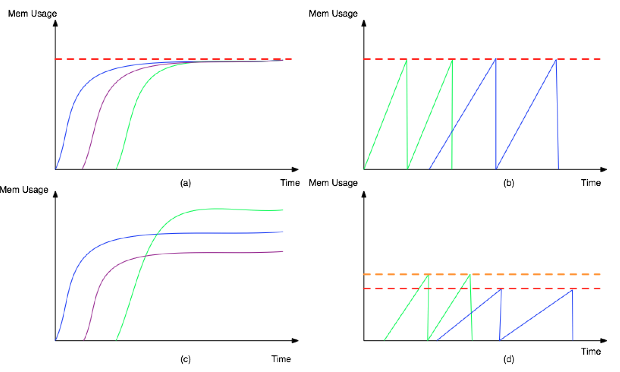
\includegraphics[width=3.0in]{image/workload.png}
    \caption{Four Memory Allocation Behaviors}
    \label{ref:memory_allocation}
\end{figure}

As shown in Figure 9(a), the X-axis red dotted line means the setting for the threshold. All the mappers have the same threshold, and will keep adding data to arraylist until it fills full up of the threshold. In this memory behavior, if the threshold is larger than the JVM maximum heap size setting, the mapper will fail and restart a new attempt with the same threshold. But mappers will start in different time as there is limit on maximum running map task slots in tasktracker. We call this behavior "Same Threshold without Clearance".

As shown in Figure 9(b), the same with the memory behaviro shown in Figure 9(a), all the map tasks have the same memory usage threshold. But the difference is that after each map task full fills its own array to threshold, it will clear all the data in the array which clears the array memory usage to 0, and then start to put data into array list again with exponential increasing speed. We call this behavior "Same Threshold with Clearance".

As shown in Figure 9(c), we can see from the line that there are different thresholds for each map task. This is the setting with the random ratio flag. The random threshold will be calculated when map task starts, and also when it fails and retries. In this case, when some of the map tasks fails due to hold large amount of data, there is chance that it can run without any problems as when it retries the theshold is much smaller than the maximum usage. We call this behavior "Random Threshold without Clearance".

We call the last one shown in Figure 9(d) "Random Threshold with Clearance". It combines the behaviors both from Figure 9(b) and Figure (c).  Every map task has its own threshold, when the data it holds reaches its own threshold, map task will clear the data in the array and then start to put data into array again until it reaches threshold and then clear data again.

